\section{Introduction and motivation}

Data visualisation is an essential component of modern data science and science
communication. Unfortunately, its power as a communicative tool means leaves it
open to both misinterpretation and misuse: patterns in raw data can be obscured,
statistical assumptions hidden, and effect sizes misrepresented
\cite{weissgerber15}. These concerns can be addressed in part through improved
statistical practices and novel plot and chart designs \cite{allen19}, but also
by making visualisations themselves more open and explorable
\cite{dragicevic19}.

One well-established technique for explorability is \emph{linked brushing}
\cite{fisherkeller75,becker87,buja91}, which allows the user to explore
interactively how a visualisation relates to other concurrent visualisations of
the same data. For example, geoscientists often work with multiple layered
views. To show how these are related, spatial analytics applications like GeoDa
\cite{anselin06} can automatically select the relevant part of one view as the
user changes the selection in a related view, say a choropleth map. Such linking
is an important navigational tool, allowing the user to switch contexts in one
view and have related views synchronise automatically. With complex multivariate
data, linking can also be an essential sense-making aid, helping the user intuit
relationships in the data \cite{he18}.

However, linked brushing and similar features usually have to be specifically
anticipated by the application or library developer. If the data analyst uses a
custom library or wants other views or visual attributes linked that the
original developer did not consider, they are out of luck. For example,
contemporary visualisation libraries for the web like Bokeh \cite{jolly18} and
D3 \cite{bostock11} provide advanced linking and brushing features, but only
through specifically designed widgets and for particular visual attributes, such
as the glyphs used to render the points in a chart.

\begin{figure}[h]
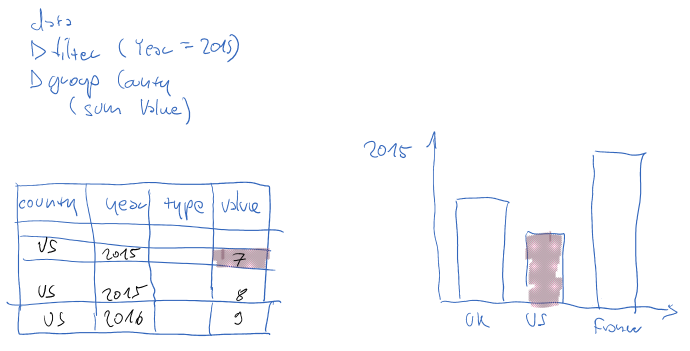
\includegraphics[scale=0.35]{image/chart-fwd}
\caption{Forward linking from code and data to visualisation}
\end{figure}

Moroever, it is our research hypothesis that, during the development of a
visualisation, it is useful to see how the visualisation relates to the
underlying data, so that one might brush over a tabular rendering of the data
code/data..debugging..transparency/reproducibility]. Roberts and Wright
identified the potential utility of ``ubiquitous brushing'' for visual elements
other than plots, such as data tables and legends \cite{roberts06}; in this
pape, we present a framework that extends linking not only to all visual
attributes but also to source code. Visualisations authored in our framework
have linking built in, making this powerful comprehension feature automatic.

We formulate the problem more precisely in \Secref{problem-overview} and
describe our solution in \Secref{framework}. \Secref{related-work} discusses
related work in more detail and \Secref{conclusion} concludes with some
directions for future work.
